\documentclass{beamer}
% \documentclass{article}
% \usepackage{beamerarticle}

\usepackage{tikz}
\usetikzlibrary{arrows.meta,arrows}
\usetikzlibrary{positioning}

\usetheme{Boadilla}
\setbeamercovered{transparent} 
\usefonttheme[onlymath]{serif}

\title{Implementation of Abstract Interpreter}
\subtitle{Software Verification Course Homework}
\author[E. Scandaletti]{Elia Scandaletti\texorpdfstring{ - 2087934\\University of Padova}{}}
\date[13/02/2023]{13th February 2023}

\begin{document}
\begin{frame}
    \titlepage
\end{frame}

\begin{frame}{Outline}
    \tableofcontents
\end{frame}

\section{Program Overview}

\begin{frame}{Program Overview}

    The program is composed of three main parts:

    \begin{block}{Parsing}
        The syntax module provides the function \texttt{build\_ast} that transform the input into an Abstract Syntax Tree.
    \end{block}

    \begin{block}{Building the Control Flow Graph}
        The Abstract Syntax Tree is then transformed in a Control Flow Graph via the \texttt{new} constructor.
    \end{block}

    \begin{block}{Abstract Execution}
        The program is abstractly executed on the control flow graph.
    \end{block}

    ~\\
    We will see each of them in detail.

\end{frame}

\section{Parsing}

\begin{frame}{Pest crate}

    The Rust crate \texttt{pest} provides a way of defining a parsing expression grammar which is then used to provide a stream of tokens given an input.

    ~\\
    The stream can be mapped recursively thanks to an utility of the same crate: the \texttt{pratt\_parser}.

    This parser arranges the tokens hierarchically in a n-ary tree.
    The number of children of a node depends on the rule corresponding to the node.
    Therefore, it's easy to convert this structure in an Abstract Syntax Tree.

\end{frame}

\begin{frame}{Abstract Syntax Tree}

    The Abstract Syntax Tree represents the structure of the input program.
    It has three types of components:
    \begin{itemize}
        \item \texttt{AExp}: represents an arithmetic expression;
        \item \texttt{BExp}: represents a boolean expression;
        \item \texttt{Stm}: represents a statement.
    \end{itemize}

    ~\\
    Each of these types is implemented as an enum.

\end{frame}

\begin{frame}{Abstract Syntax Tree}{\texttt{AExp}}

    Arithmetic expressions have multiple variants:
    \begin{itemize}
        \item \texttt{Num(\textit{n})} $\sim$ \texttt{\textit{n}};
        \item \texttt{Var(\textit{x})} $\sim$ \texttt{\textit{x}},
        \item \texttt{Add(\textit{a1}, \textit{a2})} $\sim$ \texttt{\textit{a1} + \textit{a2}};
        \item \texttt{Sub(\textit{a1}, \textit{a2})} $\sim$ \texttt{\textit{a1} - \textit{a2}};
        \item \texttt{Mul(\textit{a1}, \textit{a2})} $\sim$ \texttt{\textit{a1} * \textit{a2}};
        \item \texttt{Div(\textit{a1}, \textit{a2})} $\sim$ \texttt{\textit{a1} / \textit{a2}};
        \item \texttt{Neg(\textit{a})} $\sim$ \texttt{-\textit{a}};
        \item \texttt{PreInc(\textit{x})} $\sim$ \texttt{++\textit{x}};
        \item \texttt{PreDec(\textit{x})} $\sim$ \texttt{--\textit{x}};
        \item \texttt{PostInc(\textit{x})} $\sim$ \texttt{\textit{x}++};
        \item \texttt{PostDec(\textit{x})} $\sim$ \texttt{\textit{x}--}.
    \end{itemize}

\end{frame}

\begin{frame}{Abstract Syntax Tree}{\texttt{BExp}}

    Boolean expressions have multiple variants:
    \begin{itemize}
        \item \texttt{True} $\sim$ \texttt{true};
        \item \texttt{False} $\sim$ \texttt{false};
        \item \texttt{Eq(\textit{a1}, \textit{a2})} $\sim$ \texttt{\textit{a1} = \textit{a2}};
        \item \texttt{Neq(\textit{a1}, \textit{a2})} $\sim$ \texttt{\textit{a1} != \textit{a2}};
        \item \texttt{Lt(\textit{a1}, \textit{a2})} $\sim$ \texttt{\textit{a1} < \textit{a2}};
        \item \texttt{And(\textit{b1}, \textit{b2})} $\sim$  \texttt{\textit{b1} \&\& \textit{b2}};
        \item \texttt{Or(\textit{b1}, \textit{b2})} $\sim$ \texttt{\textit{b1} || \textit{b2}};
        \item \texttt{Not(\textit{b})} $\sim$ \texttt{!\textit{b}}.
    \end{itemize}

\end{frame}

\begin{frame}{Abstract Syntax Tree}{\texttt{Stm}}

    Statements have multiple variants:
    \begin{itemize}
        \item \texttt{AExp(id, \textit{a})} $\sim$ \textit{a}, result is ignored;
        \item \texttt{BExp(id, \textit{b})} $\sim$ \textit{b}, result is ignored;
        \item \texttt{Ass(id, \textit{x}, \textit{a})} $\sim$ \texttt{\textit{x} := \textit{a}};
        \item \texttt{Skip(id)} $\sim$ \texttt{skip};
        \item \texttt{IfThenElse(id, \textit{b}, \textit{stm}1, \textit{stm}2)} $\sim$ \\
              \hskip 1.5cm \texttt{if \textit{b} then \textit{stm}1 else \textit{stm}2 endif};
        \item \texttt{While(id, \textit{b}, \textit{stm})} $\sim$ \texttt{while \textit{b} do \textit{stm} done};
        \item \texttt{Comp(\_, \textit{stm}1, \textit{stm}2)} $\sim$ \texttt{\textit{stm}1; \textit{stm}2}.
    \end{itemize}

    ~\\
    Note that all the statements - except \texttt{Comp} -  have an id which will be used in the end for mapping the nodes in the graph to the statements.

\end{frame}

\section{Building the Control Flow Graph}

\begin{frame}{Control Flow Graph}

    The Control Flow Graph is a graph in which each vertex represents a point of a program.

    Each arc, instead, represents a command.
    A command can be either a statement or a boolean guard.

    \begin{itemize}
        \item \texttt{Guard(\textit{b})}: represents the states for which \textit{b} evaluated to true;
        \item \texttt{AExp(a)}, \texttt{BExp(b)}, \texttt{Ass(x, a)}, \texttt{Skip}: represent how the corresponding statements modify the state.
    \end{itemize}

    ~\\
    Note that the \texttt{While}, \texttt{IfThenElse} and \texttt{Comp} do not appear.
    This kinds of statement are used to build the structure of the graph.
    Their boolean guards and sub-statements become arcs of the graph.

\end{frame}

\begin{frame}{Control Flow Graph}{IfThenElse}

    \texttt{if \textit{b} then \textit{stm1} else \textit{stm2} endif}

    ~\\~\\\centering
    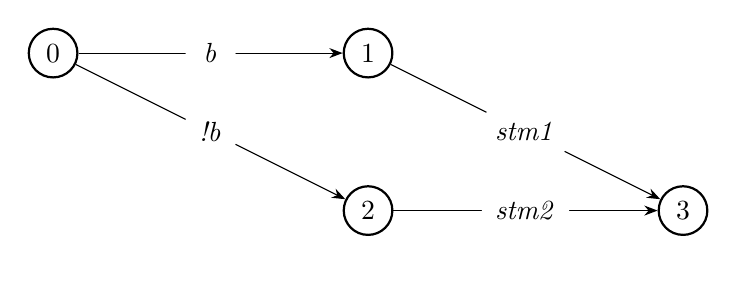
\begin{tikzpicture}

        \begin{scope}[every node/.style={circle,thick,draw}]
            \node (A) at (1,3) {0};
            \node (B) at (5,3) {1};
            \node (C) at (5,1) {2};
            \node (D) at (9,1) {3};
        \end{scope}

        \begin{scope}[>={Stealth[black]},
            every node/.style={fill=white,circle}]
            \path [->] (A) edge node {\textit{b}} (B);
            \path [->] (A) edge node {\textit{!b}} (C);
            \path [->] (B) edge node {\textit{stm1}} (D);
            \path [->] (C) edge node {\textit{stm2}} (D);
        \end{scope}
    \end{tikzpicture}

\end{frame}

\begin{frame}{Control Flow Graph}{While}

    \texttt{while \textit{b} do \textit{stm} done}

    ~\\~\\\centering
    \begin{tikzpicture}

        \begin{scope}[every node/.style={circle,thick,draw}]
            \node (A) at (3,5) {0};
            \node (B) at (1,1) {1};
            \node (C) at (7,3) {2};
        \end{scope}

        \begin{scope}[>={Stealth[black]},
            every node/.style={fill=white,circle}]
            \path [->] (A) edge[bend right=30] node {\textit{b}} (B);
            \path [->] (A) edge node {\textit{!b}} (C);
            \path [->] (B) edge[bend right=30] node {\textit{stm}} (A);
        \end{scope}
    \end{tikzpicture}

\end{frame}

\begin{frame}{Control Flow Graph}{Comp}

    \texttt{\textit{stm1}; \textit{stm2}}

    ~\\~\\\centering
    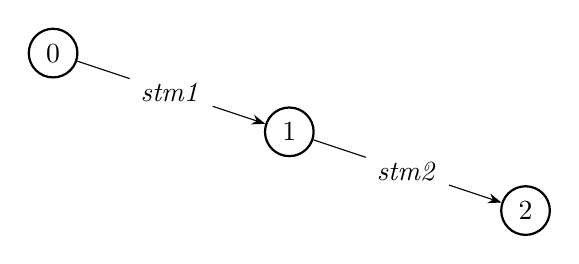
\begin{tikzpicture}

        \begin{scope}[every node/.style={circle,thick,draw}]
            \node (A) at (1,3) {0};
            \node (B) at (4,2) {1};
            \node (C) at (7,1) {2};
        \end{scope}

        \begin{scope}[>={Stealth[black]},
            every node/.style={fill=white,circle}]
            \path [->] (A) edge node {\textit{stm1}} (B);
            \path [->] (B) edge node {\textit{stm2}} (C);
        \end{scope}
    \end{tikzpicture}

\end{frame}

\section{Abstract Domain}

\begin{frame}{Bounded Intervals}

    Tha abstract domain is similar to the interval abstract domain.
    The only difference is that any value above or below two given thresholds are considered respectively $+\inf$ or $-\inf$.

    Furthermore, this domain can also represents constant values.

    \begin{multline*}
        \textrm{Int}_{m,n} = \{ \emptyset, \mathbb{Z} \}
        \cup \{ [a, b], [a, b] \subseteq [m, n] \}
        \cup \{ [k, k], k \in \mathbb{Z} \} \\
        \cup \{ (-\inf, k], k \in [m, n] \}
        \cup \{ [k, +\inf), k \in [m, n] \}
    \end{multline*}

    ~\\
    In the implementation, the empty element is represented as a special value of the interval.
    $\mathbb{Z}$, instead, is represented as the interval $(-\inf, +\inf)$.

\end{frame}

\begin{frame}{$\textrm{Int}_{m,n}$ Lattice}

    The $\textrm{Int}_{m,n}$ lattice is very similar to the interval lattice.
    In fact, it is a subset.

    ~\\

    The ordering is given by interval inclusion.

    The top element is $(-\inf, +\inf)$.
    The bottom element is $\emptyset$.

    The lub of two intervals is the smallest interval that includes both of them.

    The glb of two intervals is the intersection of the two.

    ~\\

    The abstract operations on $\textrm{Int}_{m,n}$ are defined as the operations on intervals.
    The only difference is that if a result is outside the $\textrm{Int}_{m,n}$ domain, either or both the lower and upper bound of the interval are set to $\pm \inf$.

\end{frame}

\section{Abstracting the Execution}

\begin{frame}{Abstract Execution}{Arithmetic Expressions}

    Arithmetic expressions are evaluated recursively in postfix order.

    Each evaluation has two outputs:
    \begin{itemize}
        \item the state modified by the execution;
        \item the result of the expression.
    \end{itemize}

    In the implementation, the first one is a mutable reference passed as argument.
    The second one, is the value returned by the function.

\end{frame}

\begin{frame}{Abstract Execution}{Boolean Expressions}

    Boolean expressions are evaluated recursively in postfix order.

    Each evaluation has two outputs:
    \begin{itemize}
        \item how the state is modified by the execution;
        \item the result of the expression, represented as the set of states for which the expression is true.
    \end{itemize}

    In the implementation, the first one is a mutable reference passed as argument.
    The second one, is the value returned by the function.

\end{frame}

\begin{frame}{Abstract Execution}{Boolean Expressions - Comparison Operators}

    Arithmetic expressions comparison can always be transformed in a comparison between an arithmetic expression and $0$.

    In particular: $\textit{a1} \diamond \textit{a2} \iff (\textit{a1} - \textit{a2}) \diamond 0$.

    ~\\
    The comparison is now performed in three steps:
    \begin{enumerate}
        \item building a tree of intervals corresponding to the values of each sub-expression;
        \item evaluating this tree;
        \item ``filtering'' each value such that the final tree respects the original condition.
    \end{enumerate}

\end{frame}

\begin{frame}{Abstract Execution}{Boolean Expressions - Expression Tree}

    \texttt{x := [2, 5]}

    \texttt{2 * (++x) - (x++)}

    ~\\\centering
    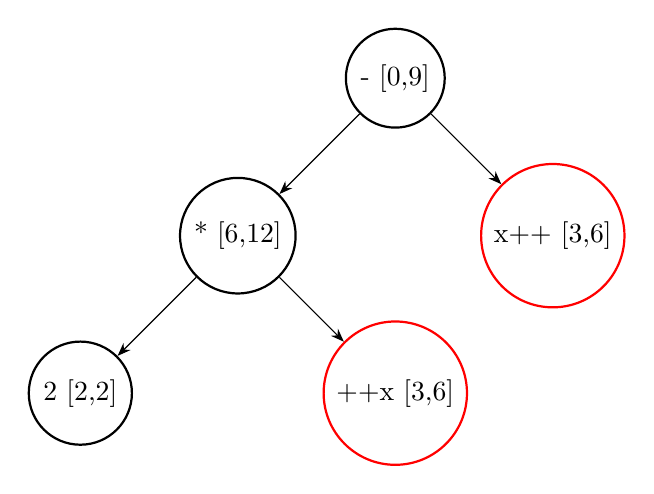
\begin{tikzpicture}

        \begin{scope}[every node/.style={circle,thick,draw}]
            \node (A) at (5,5) {- [0,9]};
            \node (B) at (3,3) {* [6,12]};
            \node (C) at (1,1) {2 [2,2]};
            \node[style={draw=red}] (D) at (5,1) {++x [3,6]};
            \node[style={draw=red}] (E) at (7,3) {x++ [3,6]};
        \end{scope}

        \begin{scope}[>={Stealth[black]}]
            \path [->] (A) edge (B);
            \path [->] (B) edge (C);
            \path [->] (B) edge (D);
            \path [->] (A) edge (E);
        \end{scope}

    \end{tikzpicture}

\end{frame}

\begin{frame}{Abstract Execution}{Boolean Expressions - Expression Tree}

    \texttt{x := [2, 5]}

    \texttt{2 * (++x) - (x++) > 5}

    ~\\\centering
    \begin{tikzpicture}

        \begin{scope}[every node/.style={circle,thick,draw}]
            \node (A) at (5,5) {- \alt<1->{[5,9]}{[0,9]}};
            \node (B) at (3,3) {* \alt<2->{[8,12]}{[6,12]}};
            \node (C) at (1,1) {2 \alt<3->{[2,2]}{[2,2]}};
            \node[style={draw=red}] (D) at (5,1) {++x \alt<5->{[4,6]}{[3,6]}};
            \node[style={draw=red}] (E) at (7,3) {x++ \alt<8->{[3,6]}{[3,6]}};
        \end{scope}

        \begin{scope}[>={Stealth[black]}]
            \path [->] (A) edge (B);
            \path [->] (B) edge (C);
            \path [->] (B) edge (D);
            \path [->] (A) edge (E);
        \end{scope}

        \begin{scope}[>={Stealth[blue]},
            every edge/.style={draw=blue}]
            \only<2->{\path [->] (A) edge[bend right=30] (B);}
            \only<3->{\path [->] (B) edge[bend right=30] (C);}
            \only<4->{\path [->] (C) edge[bend right=30] (B);}
            \only<5->{\path [->] (B) edge[bend right=30] (D);}
            \only<6->{\path [->] (D) edge[bend right=30] (B);}
            \only<7->{\path [->] (B) edge[bend right=30] (A);}
            \only<8->{\path [->] (A) edge[bend right=30] (E);}
            \only<9->{\path [->] (E) edge[bend right=30] (A);}
        \end{scope}

    \end{tikzpicture}

\end{frame}

\begin{frame}{Abstract Execution}{Boolean Expressions - \texttt{Not}}

    There are two strategies for executing the \texttt{Not} operator:
    \begin{itemize}
        \item by exploiting the De Morgan Laws and moving it towards the leaves of the boolean expression tree,\\
              e.g.: \texttt{Not(And(\textit{b1}, \textit{b2}))} $\rightarrow$ \texttt{Or(Not(\textit{b1}), Not(\textit{b2}))};
        \item by inspect the expression within and modify it in a sound way,\\
              e.g.: \texttt{Not(Eq(\textit{a1}, \textit{a2}))} $\rightarrow$ \texttt{Neq(\textit{a1}, \textit{a2})},\\
              e.g.: \texttt{Not(Not(\textit{b}))} $\rightarrow$ \texttt{\textit{b}}.
    \end{itemize}

\end{frame}

\begin{frame}{Abstract Execution}{Cahotic Iteration}

    The final task of the Abstract Interpreter is finding the invariants of each point of the program.

    In order to do so, using the Control Flow Graph, the Abstract Interpreter:
    \begin{enumerate}
        \item determines the dependencies between the invariants of different control points;
        \item put the entry point of the program in an update queue;
        \item pick the next point of the queue;
        \item calculate its invariant using the Control Flow Graph;
        \item if its invariant changed, it puts all the points that directly depends on it in the queue;
        \item if the queue is not empty, go to point 3, else finished.
    \end{enumerate}

\end{frame}

\begin{frame}
    \centering \huge
    \emph{Thank you for your attention!}
\end{frame}

\end{document}